% From <https://www.integral-domain.org/lwilliams/Resources/tikzsnippets.php>
\documentclass[tikz, usenames, dvipsnames]{standalone}
\usepackage{xstring}

\usepackage{xcolor,colortbl}
\definecolor{LightGray}{RGB}{240,240,240}
\definecolor{MLGray}{RGB}{160,160,160}
\definecolor{MedGray}{RGB}{120,120,120}
\definecolor{DarkGray}{RGB}{70,70,70}
\definecolor{Green}{RGB}{47,123,108}
\definecolor{LGreen}{RGB}{70,185,162}
\definecolor{VLGreen}{RGB}{193, 232, 224}
\definecolor{Blue}{RGB}{47,113,123}
\definecolor{LBlue}{RGB}{70,170,185}
\definecolor{Warning}{RGB}{185,85,70}
\usetikzlibrary{decorations.shapes}
\usetikzlibrary{shapes, shapes.arrows, arrows.meta}

\begin{document}
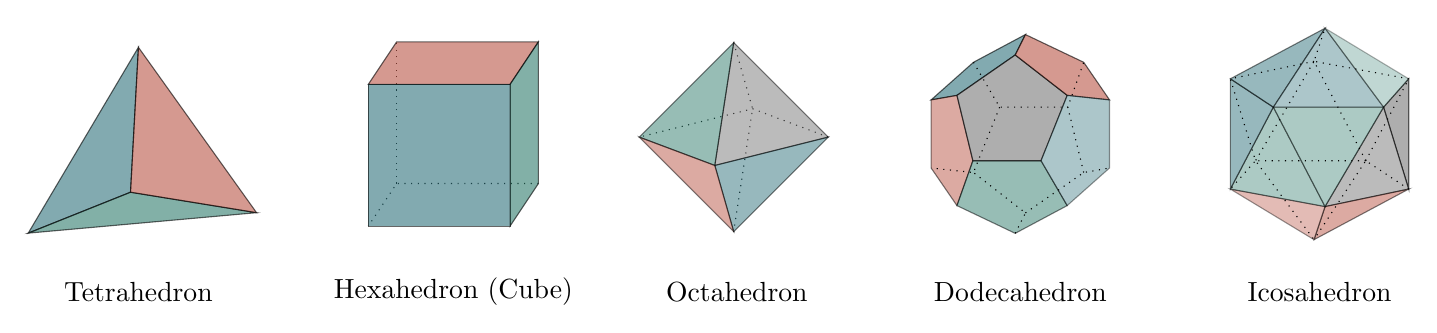
\begin{tikzpicture}
	\begin{scope}[scale=1.5,y={(-0.5cm,-0.2cm)},x={(1cm,0cm)}, z={(0cm,1.4cm)}]
	\coordinate (O) at (0, 0, 0);

	\draw[opacity=0.6,fill=Blue] (-0.5,0.866,0)--(0,0,1)--(-0.5,-0.866,0)--cycle;
	\draw[opacity=0.6,fill=Green] (1,0,0)--(-0.5,0.866,0)--(-0.5,-0.866,0)--cycle;
	\draw[opacity=0.6,fill=Warning] (0,0,1)--(1,0,0)--(-0.5,-0.866,0)--cycle;

\end{scope}
\node[inner sep = 0cm,] at (0,-1)   () {Tetrahedron};

\begin{scope}[xshift=4cm, yshift=1cm, scale=0.9,y={(0.2cm,0.3cm)},x={(1cm,0cm)}, z={(0cm,1cm)}]
	\coordinate (O) at (0, 0, 0);


	\draw[thin, dotted] (1,1,-1)--(-1,1,-1)--(-1,-1,-1);
	\draw[thin, dotted] (-1,1,-1)--(-1,1,1);

	  \draw[opacity=0.6,fill=Warning]  (1,1,1)--(1,-1,1)--(-1,-1,1)--(-1,1,1)--cycle; % top


	  \draw[opacity=0.6,fill=Blue] (1,-1,1)--(1,-1,-1)--(-1,-1,-1)--(-1,-1,1)--cycle; % front



	  \draw[opacity=0.6,fill=Green] (1,1,-1)--(1,1,1)--(1,-1,1)--(1,-1,-1)--cycle;

  \end{scope}
  \node[inner sep = 0cm,xshift=4cm] at (0,-1)   () {Hexahedron (Cube)};


  \begin{scope}[scale=1.2,xshift=6.3cm,yshift=0.8cm,y={(0.2cm,0.3cm)},x={(1cm,0cm)}, z={(0cm,1cm)}]
	\coordinate (O) at (0, 0, 0);


	\draw[thin, dotted] (1,0,0)--(0,1,0)--(-1,0,0);
	\draw[thin, dotted] (0,0,1)--(0,1,0)--(0,0,-1);

	 \draw[opacity=0.5,fill=MedGray] (1,0,0)--(0,-1,0)--(0,0,1)--cycle;
	 \draw[opacity=0.5,fill=Blue] (1,0,0)--(0,-1,0)--(0,0,-1)--cycle;
	 \draw[opacity=0.5,fill=Green] (-1,0,0)--(0,-1,0)--(0,0,1)--cycle;
	 \draw[opacity=0.5,fill=Warning] (-1,0,0)--(0,-1,0)--(0,0,-1)--cycle;
  \end{scope}
\node[inner sep = 0cm,xshift=7.6cm] at (0,-1)   () {Octahedron};


  \begin{scope}[xshift=11.2cm,yshift=1cm,scale=0.7,y={(0.15cm,0.3cm)},x={(1cm,0cm)}, z={(0cm,1cm)}]
	\coordinate (O) at (0, 0, 0);
	\pgfmathsetmacro{\gr}{1.618}
	\pgfmathsetmacro{\rg}{0.618}
	%golden ratio 1.618

	\draw[opacity=0.6,fill=Blue] (0,\rg,\gr)--(0,-\rg,\gr)--(-1,-1,1)--(-\gr,0,\rg)--(-1,1,1)--cycle; %left top
	\draw[opacity=0.5,fill=Warning] (-\gr,0,\rg)--(-1,-1,1)--(-\rg,-\gr,0)--(-1,-1,-1)--(-\gr,0,-\rg)--cycle; % left front
	\draw[opacity=0.5,fill=Green] (-\rg,-\gr,0)--(\rg,-\gr,0)--(1,-1,-1)--(0,-\rg,-\gr)--(-1,-1,-1)--cycle;  %lower front
	\draw[opacity=0.6,fill=MedGray] (0,-\rg,\gr)--(1,-1,1)--(\rg,-\gr,0)--(-\rg,-\gr,0)--(-1,-1,1)--cycle; %center front
	\draw[opacity=0.6,fill=Warning] (0,\rg,\gr)--(1,1,1)--(\gr,0,\rg)--(1,-1,1)--(0,-\rg,\gr)--cycle; %right top
	\draw[opacity=0.4,fill=Blue] (1,-1,1)--(\gr,0,\rg)--(\gr,0,-\rg)--(1,-1,-1)--(\rg,-\gr,0)--cycle; %right



	\draw[thin, dotted] (-1,1,1)--(-\rg,\gr,0)--(\rg,\gr,0)--(1,1,1);
	\draw[thin, dotted] (-\rg,\gr,0)--(-1,1,-1)--(-\gr,0,-\rg);
	\draw[thin, dotted] (0,-\rg,-\gr)--(0,\rg,-\gr)--(-1,1,-1);
	\draw[thin, dotted] (0,\rg,-\gr)--(1,1,-1)--(\gr,0,-\rg);
	\draw[thin, dotted] (1,1,-1)--(\rg,\gr,0);
  \end{scope}
\node[inner sep = 0cm,xshift=11.2cm] at (0,-1)   () {Dodecahedron};

  \begin{scope}[xshift=15cm,yshift=1cm,scale=0.7,y={(0.1cm,0.3cm)},x={(1cm,0cm)}, z={(0cm,1cm)}]
	\coordinate (O) at (0, 0, 0);
	\pgfmathsetmacro{\gr}{1.618}
	%golden ratio 1.618



	\draw[opacity=0.6,fill=MedGray] (\gr,0,1)--(1,\gr,0)--(\gr,0,-1)--cycle;     % right right
	\draw[opacity=0.5,fill=MedGray] (0,1,-\gr)--(1,\gr,0)--(\gr,0,-1)--cycle;    %right front
	\draw[opacity=0.5,fill=Warning] (0,1,-\gr)--(0,-1,-\gr)--(\gr,0,-1)--cycle;  %lower right
	\draw[opacity=0.4,fill=Warning] (0,1,-\gr)--(0,-1,-\gr)--(-\gr,0,-1)--cycle; %lower left
	\draw[opacity=0.4,fill=Green] (0,1,-\gr)--(-1,\gr,0)--(-\gr,0,-1)--cycle; %center left
	\draw[opacity=0.4,fill=Green] (0,1,-\gr)--(-1,\gr,0)--(1,\gr,0) --cycle; %center right
	\draw[opacity=0.5,fill=Blue] (-\gr,0,1) --(-1,\gr,0)--(-\gr,0,-1)--cycle; %left left
	\draw[opacity=0.5,fill=Blue] (-\gr,0,1) --(-1,\gr,0)--(0,1,\gr)--cycle; %top left
	\draw[opacity=0.4,fill=Blue] (1,\gr,0) --(-1,\gr,0)--(0,1,\gr)--cycle; %top center
	\draw[opacity=0.3,fill=Green] (1,\gr,0) --(\gr,0,1)--(0,1,\gr)--cycle; %top right

	\draw[thin, dotted] (0,-1,\gr)--(-\gr,0,1)--(-1,-\gr,0)--(-\gr,0,-1) ;
	\draw[thin, dotted] (\gr,0,1) --(0,-1,\gr)--(0,1,\gr);
	\draw[thin, dotted] (\gr,0,-1)--(1,-\gr,0)--(0,-1,-\gr);
	\draw[thin, dotted] (1,-\gr,0)--(-1,-\gr,0)--(0,-1,-\gr);
	\draw[thin, dotted] (1,-\gr,0) --(\gr,0,1);
	\draw[thin, dotted] (1,-\gr,0)--(0,-1,\gr)--(-1,-\gr,0);

  \end{scope}
  \node[inner sep = 0cm,xshift=15cm] at (0,-1)   () {Icosahedron};
\end{tikzpicture}
\end{document}
